\title{Report on \\ Model Development for Fossil Fuel Divestment}
\author{Jakob J. Kolb \\ Potsdam Institute for Climate Impact Research}

\maketitle

\section{Model Development}

Previous studies \cite{Ans2013} suggest that feedback through supply-demand price mechanisms will have only limited impact on fossil fuel companies. This is due to the fact, that only approximately 15 \% of investors invest subject to socially responsible guidelines \cite{SIF2014Report} and that divested holdings are, especially in liquid markets, very likely to quickly find their way to less responsible investors. \\
Therefore, the effects of a divestment campaigns on target industries rather stem from `soft' factors such as changes in market norms and stigmatization and growing uncertainty about future business opportunities. This means that for the understanding of the campaign dynamics, opinion spreading with respect to beliefs about future business development and respective uncertainties amongst investors might be worth a closer look. \\
In the following I propose a preliminary scheme of such a model.

\begin{figure}[h]
	\centering
	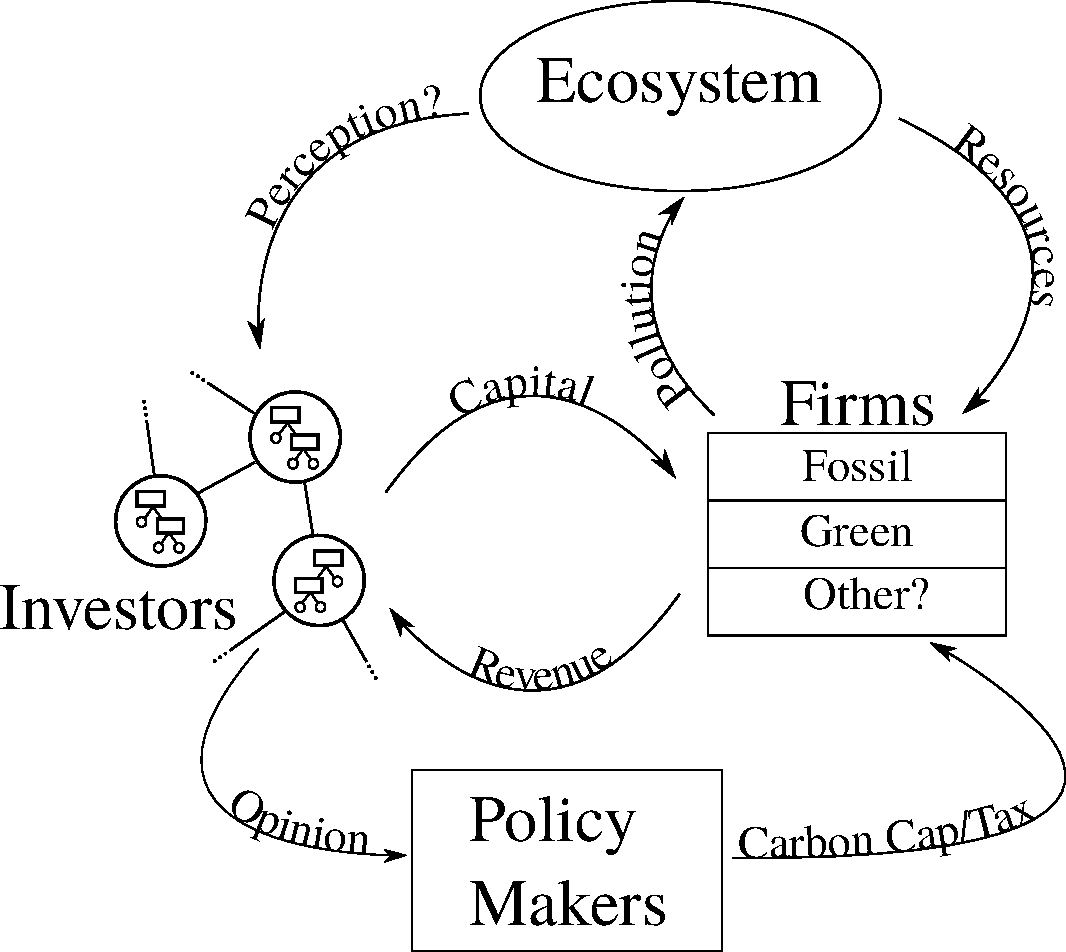
\includegraphics[width = .7 \textwidth]{Model_Scheme.pdf}
	\caption{Schematic sketch of the model including four major components: Households, Firms (grouped by sector), Ecosystem and optional Policy makers.}
	\label{fig:model}
\end{figure}

\subsection{Ramsey-Cass-Koopmans Model of optimal saving}


\subsection{Sectors}

Production is assumed to take place in two sectors. One sector $(d)$ employs a dirty technology depending on fossil resources, the other sector $(c)$ employs a clean technology relying on renewable resources. Both sectors use capital $K_j$ and labor $L$ as input factors, the dirty sector additionally uses a fossil resource $R$.
\begin{equation}
	Y_j = F_j(K_j,L,R), \qquad \frac{\partial F_c}{\partial R} = 0 	
	\label{eq:production}
\end{equation}
The total cost for fossil resource extraction $c_R$ (exploration and exploitation) is assumed to scale with the square of the resource uptake. The factor $\rho$ is presumably depending on the remaining Fossil resource and increasing as the remaining resource decreases. Also, for optimal production, resource uptake is adjusted such that the extraction costs are equal to the marginal productivity of the resource:
\begin{equation}
	c_R = \rho R_{d}^{2}, \qquad c_R = \frac{\partial F_d}{\partial R_d}
	\label{resource_extraction_cost}
\end{equation}
Capital is bound to the respective technology implemented. For high [low] intensity of fossil resource use, i.e. $R \gg 1$ [$R \ll 1$], productivities of other input factors are assumed to be higher [lower] in the dirty sector compared to the clean sector:
\begin{align}
	R \gg 1 \quad \Rightarrow & \quad \frac{\partial F_d}{\partial K_d} > \frac{\partial F_c}{ \partial K_c}, \quad \frac{\partial F_d}{\partial L} > \frac{\partial F_c}{ \partial L}, \\
	R \ll 1 \quad \Rightarrow & \quad \frac{\partial F_d}{\partial K_d} < \frac{\partial F_c}{ \partial K_c}, \quad \frac{\partial F_d}{\partial L} < \frac{\partial F_c}{ \partial L}.
	\label{eq:input_factor_productivities}
\end{align}
For the input factor markets, market clearing is assumed. Capital rental rate and wages are thereby determined by marginal factor productivities of the respective input factors.
For the wage rate, this results in the following conditions:
\begin{equation}
	\left. \frac{\partial F_d}{ \partial L} \right|_{L_d} = \left. \frac{\partial F_c}{\partial L}\right|_{L_c} = w, \qquad L_d + L_c = \sum_i L_i
	\label{eq:wage_rage}
\end{equation}
and for the capital rental rate this results in the following conditions:
\begin{align}
	\left. \frac{\partial F_d}{\partial K}\right|_{K_d} &= r_d,\quad K_d = \sum_i K^{(d)}_i \nonumber \\
	\left. \frac{\partial F_c}{\partial K}\right|_{K_c} &= r_c,\quad K_c = \sum_i K^{(c)}_i 
	\label{eq:capital_rental_rate}
\end{align}


\subsection{Households}

\textbf{Income and savings accounting:} \\
Households denoted with the Index $i$, $i \in [1, \dots N]$ are are owners of capital $A$ as well as suppliers of labor $L$. A household has $L_i$ members, each supplying one unit of labor per unit of time $t$. The wealth $A_i$ of the household is generated by labor income, capital returns and is diminished by consumption and capital depreciation:
\begin{equation}
	\dot{A}_i = \sum_j r_j K^{(j)}_{i} + wL -c_{i}L_i - \sum_j \delta_j K^{(j)}_{i}
	\label{eq:household_wealth}
\end{equation}
where $r_j$ and $\delta_j$ are the rates of return and depreciation of capital of type $K_j$, $w$ is the wage rate and $c_i$ is the consumption per member of household $i$. Capital goods are linked to either clean or dirty technology indicated with the indices $c$ and $d$. Since there is only these two capital goods available,
\begin{equation}
	A_i = K^{(c)}_{i} + K^{(d)}_{i}
	\label{eq:household_capital}
\end{equation}

\textit{ Until further notice, capital investment is considered irretrievable and capital can not be resold for consumption, e.g. the households decision making is subject to the constraint that its savings rate is bounded from below: $\sum_j r_j K^{(j)}_{i} + wL -c_{i}L_i = s \ge 0$. Down the road, trading of capital amongst households might be considered.} \\

\textbf{Savings investment - decision making:} \\
Households have two degrees of freedom that they have to decide upon. They can set their consumption level $c$ and they have to decide in which of the two capital goods they want to invest their savings. These decision processes are assumed to be bounded rational and are implemented in the framework of Fast and Frugal Heuristics.\\
Decision cues are:
\begin{table}[H]
	\centering
	\begin{tabular}{ll}
		$ROI = \frac{r_j(t)}{\delta_j}$ & total return of investment over lifetime according to current return rate,\\
		$DR = E_{t-\Delta t, t}[\dot{r}_j]$ & Dynamics of rate of return in sector $j$ during previous investment period, \\
		$MORAL$ & Whether the investment is clean or dirty, \\
		$GROUP$ & majority vote amongst neighbors. \\
	\end{tabular}
	\caption{Definition of investment decision cues}
	\label{tab:decision_cues}
\end{table}

\textit{Open questions}
\begin{itemize}
	\item Exact definition of decision problem e.g. binary choice? satisficing and accept/reject with fast and frugal tree?
\end{itemize}

\textbf{Opinion formation and social dynamics:} \\
The structure of the decision heuristics is interpreted as preferences/opinions resulting from conceptual social dynamic. \\
Technically, this means that households are connected by a social network. Households are nodes, connections are links. Every household has equal probability per time to become `active' and
\begin{itemize}
	\item chose one of his neighbors to compare himself to,
	\item compare a fitness parameter (some combination of income, wealth and consumption level) if higher, adopt the neighbors decision strategy, if lower cut link and connect to new neighbor with similar fitness.
	\item then based on the resulting behavioral parameters, decide upon consumption level and the type of capital to invest in during the next `inactive' period.
\end{itemize}

For now, the fitness parameter will be income. Later, I will try some combination of income and consumption, is likely to prevent the spreading of strategies that lead to over-saving.\\
So the fitness of household $i$ is equal to
\begin{equation}
	W_i = \sum_j r_j K^{(j)}_{i} + wL
	\label{eq:fitness}
\end{equation}

\textit{Open questions}
\begin{itemize}
	\item Further definitions of fitness parameter,
	\item Exact definition of consumption adjustment.
\end{itemize}

\subsection{Ecosystem}
Ecosystem is the source of resources and the sink for pollution. Minimal implementation would be a fixed carbon stock that is exploited by the fossil fuel sector. Optionally one could implement some sort of climate impact as a consequence of pollution.

\subsection{Policy Makers}
Policy makers can implement some carbon tax or carbon cap on economy to incentivize green development. The implementation of such measure depends on the prevalence of opinions amongst voters (are investors a representative sample of voters?) and might be appropriately implemented by a Poisson distributed random variable.

\subsection{Variables}

\begin{table}[H]
	\centering
	\begin{tabular}{r|l}
		Variable & Description \\\hline
		$A_i(t)$ & Wealth of household, $i$ \\
		$L_i(t)$ & Members of household, $i$ \\
		$a_i(t)$ & Wealth per member of household, $i$ \\
		$A_i^{(j)} (t)$ & Capital of household $i$ in sector $j$, \\
		$w(t)$   & Wage rate, \\
		$r_j(t)$ & Capital return rate in sector $j$, \\
		$c_R(t)$ & Fossil resource extraction cost, \\
		$Y_j(t)$ & Output of sector, $j$ \\
		$L_j(t)$ & total labor employed in sector $j$, \\
		$K_j(t)$ & Total capital employed in sector $j$, \\
		$R_j(t)$ & Total amount of resources consumed by sector $j$ during time $[t, t + \Delta t]$. \\
	\end{tabular}
	\caption{Variables of the model with description.}
	\label{tab:variables}
\end{table}

\subsection{Parameters}

\begin{table}[H]
	\centering
	\begin{tabular}{r|l}
		Parameter & Description \\\hline
		
	\end{tabular}
	\caption{Parameters of the model with description.}
	\label{tab:parameters}
\end{table}


\section{Implementation}

Lets assume a Cobb Douglas production function:
\begin{equation}
	F_j(K_j,L_j,R_j,t) = C(t)K_j^{\alpha_j}L_j^{\beta_j}R_j^{\gamma_j}, \qquad j = c,d.
	\label{cobb_douglas}
\end{equation}
with $\alpha_j + \beta_j + \gamma_j = 1$ to maintain economies of scale. For the clean sector, $\gamma_c = 0$ since it does not depend on the fossil resource.
Then, the economic development is subject to the following equations:\\

Market clearing for labor $L$:

\begin{equation}
	L_c + L_d = \sum_i L_i, \qquad w = C(t)K_c^{\alpha_c}(1-\alpha_c) L_c^{-\alpha_c}=  C(t)K_d^{\alpha_d}\beta_d L_d^{\beta_d-1}R_d^{1-\alpha_d - \beta_d} 
	\label{labour_market_clearing}
\end{equation}

\begin{itemize}
	\item THESE EQUATIONS NEED TO BE SOLVED EXPLICITLY
\end{itemize}

Market clearing for capital $K$:

\begin{align}
	&K_c = \sum_i K_i^{(c)}, \quad r_c = C(t)\alpha_c K_c^{\alpha_c-1} L_c^{1-\alpha_c}, \\
	&K_d = \sum_i K_i^{(d)}, \quad r_d = C(t)\alpha_d K_d^{\alpha_d-1} L_d^{\beta_d}R_d^{1-\alpha_d - \beta_d}.
	\label{capital_market_clearing}
\end{align}

The equation for the household income couples the dynamics of the household variables to each other:

\begin{equation}
	I_i = r_c K_i^{(c)} + r_d K_i^{(d)} + wL_i
	\label{household_income}
\end{equation}

Capital return rate and wages act as a 'mean field' since they are set by the market clearing conditions according to marginal returns at the cumulated supply of the respective input factors. \\

Household investment is subject to the decision parameter $x_i \in [c,d]$ and the consumption level of the household:
\begin{align}
	\dot{K}_i^{(c)} &= \delta(x_i-c)I_i(1-c_i) \\
	\dot{K}_i^{(d)} &= \delta(x_i-d)I_i(1-c_i)
	\label{household_investment}
\end{align}

\textit{If decision parameters are random/fixed, the economic model can be implemented as a stand alone.
Therefore, I will need to find an efficient way to integrate the given set of ordinary coupled differential equations.}

If eq. \eqref{household_income} is substituted in eq. \eqref{household_investment}, the combined equations read:

\begin{align}
	\dot{K}_i^{(c)} &= \delta(x_i-c)(r_c K_i^{(c)} + r_d K_i^{(d)} + wL_i)(1 -c_i) \\
	\dot{K}_i^{(d)} &= \delta(x_i-d)(r_c K_i^{(c)} + r_d K_i^{(d)} + wL_i)(1 -c_i)
	\label{household_capital_dynamics}
\end{align}

These equations can be discretized in time:

\begin{align}
	K_i^{(c)}(t + \Delta t) &= K_{i}^{(c)}(t) + \delta(x_i-c)(r_c K_i^{(c)} + r_d K_i^{(d)} + wL_i)(1 -c_i)\Delta t \\
	K_i^{(d)}(t + \Delta t) &= K_{i}^{(d)}(t) + \delta(x_i-d)(r_c K_i^{(c)} + r_d K_i^{(d)} + wL_i)(1 -c_i)\Delta t
	\label{household_capital_dynamics_discretized}
\end{align}

And the system can be integrated by evaluating the market clearing conditions \eqref{labour_market_clearing} and \eqref{capital_market_clearing} at each time step.

\bibliography{PhD-Divestment.bib}{}
    \bibliographystyle{IEEEtran}
